% !TeX root = ../../thesis.tex
\chapter{Supplementary materials: HBV Phylogeography}
\label{appendix_ch3}

Data and code used in this project are available on GitHub (\url{https://github.com/barneypotter24/hbv_phylogeography}).
% Please add the following required packages to your document preamble:
% \usepackage{multirow}
\begin{sidewaystable}[htp]
    \begin{tabular}{|l|l|ll|}
    \hline
    \multirow{2}{*}{Socio-demographic characteristics} & Men (\%) & \multicolumn{2}{l|}{96 (72\%)} \\ \cline{2-4} 
     & Age (years) median {[}IQR{]} & \multicolumn{2}{l|}{30 {[}25-37{]}} \\ \hline
    \multirow{5}{*}{Serology} & HIV co-infection (\%)* & \multicolumn{2}{l|}{19 (14\%)} \\ \cline{2-4} 
     & HCV co-infection (\%)* & \multicolumn{2}{l|}{3 (2\%)} \\ \cline{2-4} 
     & Positive eAg (\%) & \multicolumn{2}{l|}{78 (58.65\%)} \\ \cline{2-4} 
     & Positive eAb (\%) & \multicolumn{2}{l|}{63 (47.37\%)} \\ \cline{2-4} 
     & Positive Anti-HBs (\%)** & \multicolumn{2}{l|}{3 (2.34\%)} \\ \hline
    \multirow{10}{*}{\begin{tabular}[c]{@{}l@{}}Genotypes\\ (n, \%)\end{tabular}} & \multirow{4}{*}{\begin{tabular}[c]{@{}l@{}}A\\ (55, 41.35\%)\end{tabular}} & \multicolumn{1}{l|}{A1} & 33 (24.7\%) \\ \cline{3-4} 
     &  & \multicolumn{1}{l|}{A2} & 1 (0.75\%) \\ \cline{3-4} 
     &  & \multicolumn{1}{l|}{A3 Quasi-subgenotype} & 14 (10.52\%) \\ \cline{3-4} 
     &  & \multicolumn{1}{l|}{A6} & 7 (5.26\%) \\ \cline{2-4} 
     & \multirow{3}{*}{\begin{tabular}[c]{@{}l@{}}D\\ (8, 6.0\%)\end{tabular}} & \multicolumn{1}{l|}{D1} & 5 (3.75\%) \\ \cline{3-4} 
     &  & \multicolumn{1}{l|}{D2} & 2 (1.5\%) \\ \cline{3-4} 
     &  & \multicolumn{1}{l|}{D7} & 1 (0.75\%) \\ \cline{2-4} 
     & \begin{tabular}[c]{@{}l@{}}E \\ (67, 50.25\%)\end{tabular} & \multicolumn{1}{l|}{E} & 67 (50.25\%) \\ \cline{2-4} 
     & \multirow{2}{*}{\begin{tabular}[c]{@{}l@{}}Recombinant forms\\ (3, 2.25\%)\end{tabular}} & \multicolumn{1}{l|}{A/E} & 1 (0.75\%) \\ \cline{3-4} 
     &  & \multicolumn{1}{l|}{D/E} & 2 (1.5\%) \\ \hline
    \end{tabular}
    \caption{Socio-demographic and clinical characteristics of the 133 HBV-infected individuals in our study. $^*$One study participant was not tested for both HIV and HCV. $^{**}$ Based on 128 cases, data not available for 5 individuals}
    \label{suptab:hbv-s1}
    \end{sidewaystable}


    % Please add the following required packages to your document preamble:
% \usepackage{multirow}
\begin{sidewaystable}[htp]
    \resizebox{\columnwidth}{!}{
    \begin{tabular}{|l|llllllllll|l|}
    \hline
    \multirow{3}{*}{Country of origin} & \multicolumn{10}{l|}{HBV Genotype and subgenotypes (\%)} & \multirow{3}{*}{Total (\%)} \\ \cline{2-11}
     & \multicolumn{5}{l|}{\begin{tabular}[c]{@{}l@{}}A\\ (n=55, 41.4\%)\end{tabular}} & \multicolumn{3}{l|}{\begin{tabular}[c]{@{}l@{}}D\\ (n= 8, 6\%)\end{tabular}} & \multicolumn{1}{l|}{\multirow{2}{*}{\begin{tabular}[c]{@{}l@{}}E\\ (n=67, 50.4\%)\end{tabular}}} & \multirow{2}{*}{\begin{tabular}[c]{@{}l@{}}Recombinant forms\\ (n=3, 2.2\%)\end{tabular}} &  \\ \cline{2-9}
     & \multicolumn{1}{l|}{A1} & \multicolumn{1}{l|}{A2} & \multicolumn{1}{l|}{A3*} & \multicolumn{1}{l|}{A5*} & \multicolumn{1}{l|}{A6} & \multicolumn{1}{l|}{D1} & \multicolumn{1}{l|}{D2} & \multicolumn{1}{l|}{D7} & \multicolumn{1}{l|}{} &  &  \\ \hline
    Angola & \multicolumn{1}{l|}{0} & \multicolumn{1}{l|}{0} & \multicolumn{1}{l|}{1} & \multicolumn{1}{l|}{0} & \multicolumn{1}{l|}{0} & \multicolumn{1}{l|}{0} & \multicolumn{1}{l|}{0} & \multicolumn{1}{l|}{0} & \multicolumn{1}{l|}{0} & 0 & 1   (0.75) \\ \hline
    Burkina Faso/Togo & \multicolumn{1}{l|}{0} & \multicolumn{1}{l|}{0} & \multicolumn{1}{l|}{0} & \multicolumn{1}{l|}{0} & \multicolumn{1}{l|}{0} & \multicolumn{1}{l|}{0} & \multicolumn{1}{l|}{0} & \multicolumn{1}{l|}{0} & \multicolumn{1}{l|}{1} & 0 & 1   (0.75) \\ \hline
    Burundi & \multicolumn{1}{l|}{3} & \multicolumn{1}{l|}{0} & \multicolumn{1}{l|}{0} & \multicolumn{1}{l|}{0} & \multicolumn{1}{l|}{0} & \multicolumn{1}{l|}{0} & \multicolumn{1}{l|}{0} & \multicolumn{1}{l|}{0} & \multicolumn{1}{l|}{1} & 0 & 4	(3.0) \\ \hline
    Cameroon & \multicolumn{1}{l|}{0} & \multicolumn{1}{l|}{0} & \multicolumn{1}{l|}{2} & \multicolumn{1}{l|}{0} & \multicolumn{1}{l|}{0} & \multicolumn{1}{l|}{0} & \multicolumn{1}{l|}{0} & \multicolumn{1}{l|}{0} & \multicolumn{1}{l|}{8} & 0 & 10  (7.52) \\ \hline
    Congo & \multicolumn{1}{l|}{15} & \multicolumn{1}{l|}{1} & \multicolumn{1}{l|}{3} & \multicolumn{1}{l|}{2} & \multicolumn{1}{l|}{7} & \multicolumn{1}{l|}{2} & \multicolumn{1}{l|}{1} & \multicolumn{1}{l|}{1} & \multicolumn{1}{l|}{12} & 0 & 44  (33.0) \\ \hline
    Ghana & \multicolumn{1}{l|}{0} & \multicolumn{1}{l|}{0} & \multicolumn{1}{l|}{0} & \multicolumn{1}{l|}{0} & \multicolumn{1}{l|}{0} & \multicolumn{1}{l|}{1} & \multicolumn{1}{l|}{0} & \multicolumn{1}{l|}{0} & \multicolumn{1}{l|}{3} & 0 & 4	(3.0) \\ \hline
    Guinea & \multicolumn{1}{l|}{0} & \multicolumn{1}{l|}{0} & \multicolumn{1}{l|}{1} & \multicolumn{1}{l|}{0} & \multicolumn{1}{l|}{0} & \multicolumn{1}{l|}{0} & \multicolumn{1}{l|}{0} & \multicolumn{1}{l|}{0} & \multicolumn{1}{l|}{19} & 1 & 21  (15.75) \\ \hline
    Ivory Coast & \multicolumn{1}{l|}{0} & \multicolumn{1}{l|}{0} & \multicolumn{1}{l|}{1} & \multicolumn{1}{l|}{0} & \multicolumn{1}{l|}{0} & \multicolumn{1}{l|}{0} & \multicolumn{1}{l|}{0} & \multicolumn{1}{l|}{0} & \multicolumn{1}{l|}{6} & 0 & 7	(5.26) \\ \hline
    Mauritania & \multicolumn{1}{l|}{0} & \multicolumn{1}{l|}{0} & \multicolumn{1}{l|}{1} & \multicolumn{1}{l|}{0} & \multicolumn{1}{l|}{0} & \multicolumn{1}{l|}{0} & \multicolumn{1}{l|}{0} & \multicolumn{1}{l|}{0} & \multicolumn{1}{l|}{5} & 0 & 6	(4.51) \\ \hline
    Mozambique & \multicolumn{1}{l|}{0} & \multicolumn{1}{l|}{0} & \multicolumn{1}{l|}{0} & \multicolumn{1}{l|}{0} & \multicolumn{1}{l|}{0} & \multicolumn{1}{l|}{0} & \multicolumn{1}{l|}{0} & \multicolumn{1}{l|}{0} & \multicolumn{1}{l|}{1} & 0 & 1	(0.75) \\ \hline
    Niger & \multicolumn{1}{l|}{0} & \multicolumn{1}{l|}{0} & \multicolumn{1}{l|}{0} & \multicolumn{1}{l|}{0} & \multicolumn{1}{l|}{0} & \multicolumn{1}{l|}{1} & \multicolumn{1}{l|}{0} & \multicolumn{1}{l|}{0} & \multicolumn{1}{l|}{4} & 0 & 5	(3.75) \\ \hline
    Nigeria & \multicolumn{1}{l|}{0} & \multicolumn{1}{l|}{0} & \multicolumn{1}{l|}{1} & \multicolumn{1}{l|}{0} & \multicolumn{1}{l|}{0} & \multicolumn{1}{l|}{0} & \multicolumn{1}{l|}{0} & \multicolumn{1}{l|}{0} & \multicolumn{1}{l|}{2} & 0 & 3	(2.26) \\ \hline
    Rwanda & \multicolumn{1}{l|}{15} & \multicolumn{1}{l|}{0} & \multicolumn{1}{l|}{1} & \multicolumn{1}{l|}{0} & \multicolumn{1}{l|}{0} & \multicolumn{1}{l|}{1} & \multicolumn{1}{l|}{1} & \multicolumn{1}{l|}{0} & \multicolumn{1}{l|}{3} & 2 & 23  (17.25) \\ \hline
    Senegal & \multicolumn{1}{l|}{0} & \multicolumn{1}{l|}{0} & \multicolumn{1}{l|}{0} & \multicolumn{1}{l|}{0} & \multicolumn{1}{l|}{0} & \multicolumn{1}{l|}{0} & \multicolumn{1}{l|}{0} & \multicolumn{1}{l|}{0} & \multicolumn{1}{l|}{1} & 0 & 1	(0.75) \\ \hline
    Zimbabwe & \multicolumn{1}{l|}{0} & \multicolumn{1}{l|}{0} & \multicolumn{1}{l|}{0} & \multicolumn{1}{l|}{0} & \multicolumn{1}{l|}{0} & \multicolumn{1}{l|}{0} & \multicolumn{1}{l|}{0} & \multicolumn{1}{l|}{0} & \multicolumn{1}{l|}{1} & 0 & 1	(0.75) \\ \hline
    Unknown & \multicolumn{1}{l|}{0} & \multicolumn{1}{l|}{0} & \multicolumn{1}{l|}{1} & \multicolumn{1}{l|}{0} & \multicolumn{1}{l|}{0} & \multicolumn{1}{l|}{0} & \multicolumn{1}{l|}{0} & \multicolumn{1}{l|}{0} & \multicolumn{1}{l|}{0} & 0 & 1	(0.75) \\ \hline
    Total (\%) & \multicolumn{1}{l|}{\begin{tabular}[c]{@{}l@{}}33\\ (24.7)\end{tabular}} & \multicolumn{1}{l|}{\begin{tabular}[c]{@{}l@{}}1\\ (0.75)\end{tabular}} & \multicolumn{1}{l|}{\begin{tabular}[c]{@{}l@{}}12\\ (9.0)\end{tabular}} & \multicolumn{1}{l|}{\begin{tabular}[c]{@{}l@{}}2\\ (1.5)\end{tabular}} & \multicolumn{1}{l|}{\begin{tabular}[c]{@{}l@{}}7\\ (5.26)\end{tabular}} & \multicolumn{1}{l|}{\begin{tabular}[c]{@{}l@{}}5\\ (3.75)\end{tabular}} & \multicolumn{1}{l|}{\begin{tabular}[c]{@{}l@{}}2\\ (1.5)\end{tabular}} & \multicolumn{1}{l|}{\begin{tabular}[c]{@{}l@{}}1\\ (0.75)\end{tabular}} & \multicolumn{1}{l|}{\begin{tabular}[c]{@{}l@{}}67\\ (50.25)\end{tabular}} & \begin{tabular}[c]{@{}l@{}}3\\ (2.25)\end{tabular} & \begin{tabular}[c]{@{}l@{}}133\\ (100\%)\end{tabular} \\ \hline
    \end{tabular}
    }
    \caption{Frequencies of HBV genotypes and subgenotypes according to the countries of origin. $^*$Cluster as Quasi-subgenotypes A3.}
    \label{suptab:hbv-s2}
    \end{sidewaystable}

% Please add the following required packages to your document preamble:
% \usepackage{multirow}
% \usepackage{longtable}
% Note: It may be necessary to compile the document several times to get a multi-page table to line up properly
\clearpage
\begingroup\footnotesize
\begin{longtable}{|l|l|l|lll|}
    \hline
    \multirow{2}{*}{Gene} & \multirow{2}{*}{Mutation} & \multirow{2}{*}{n (\%)} & \multicolumn{3}{l|}{\begin{tabular}[c]{@{}l@{}}Genotype*\\ OR \\ {[}95\% CI{]}\end{tabular}} \\ \cline{4-6} 
     &  &  & \multicolumn{1}{l|}{A} & \multicolumn{1}{l|}{D} & E \\ \hline
    \endfirsthead
    %
    \endhead
    %
    \multirow{19}{*}{core} & 1653 & 15 (11.28) & \multicolumn{1}{l|}{\begin{tabular}[c]{@{}l@{}}0.317 \\ {[}0.085-1.183{]}\end{tabular}} & \multicolumn{1}{l|}{-} & \begin{tabular}[c]{@{}l@{}}4.581 \\ {[}1.229-17.08{]}*\end{tabular} \\ \cline{2-6} 
     & 1762 & 40 (30.08) & \multicolumn{1}{l|}{\begin{tabular}[c]{@{}l@{}}0.422 \\ {[}0.188-0.944{]}*\end{tabular}} & \multicolumn{1}{l|}{\begin{tabular}[c]{@{}l@{}}1.427\\ {[}0.324-6.281\end{tabular}} & \begin{tabular}[c]{@{}l@{}}2.355\\ {[}1.092-5.076{]}*\end{tabular} \\ \cline{2-6} 
     & 1764 & 49 (36.84) & \multicolumn{1}{l|}{\begin{tabular}[c]{@{}l@{}}0.965 \\ {[}0.471-1.975{]}\end{tabular}} & \multicolumn{1}{l|}{\begin{tabular}[c]{@{}l@{}}1.777 \\ {[}0.424-7.452{]}\end{tabular}} & \begin{tabular}[c]{@{}l@{}}0.915 \\ {[}0.452-1.852{]}\end{tabular} \\ \cline{2-6} 
     & 1766 & 18 (13.53) & \multicolumn{1}{l|}{\begin{tabular}[c]{@{}l@{}}2.535 \\ {[}0.914-7.028{]}\end{tabular}} & \multicolumn{1}{l|}{-} & \begin{tabular}[c]{@{}l@{}}0.442 \\ {[}0.155-1.260{]}\end{tabular} \\ \cline{2-6} 
     & 1858 & \begin{tabular}[c]{@{}l@{}}7 \\ (5.26)\end{tabular} & \multicolumn{1}{l|}{\begin{tabular}[c]{@{}l@{}}3.8 \\ {[}0.709-20.352{]}\end{tabular}} & \multicolumn{1}{l|}{-} & \begin{tabular}[c]{@{}l@{}}0.151 \\ {[}0.017-1.295{]}*\end{tabular} \\ \cline{2-6} 
     & 1896 & 34 (25.56) & \multicolumn{1}{l|}{\begin{tabular}[c]{@{}l@{}}0.087 \\ {[}0.025-0.304{]}*\end{tabular}} & \multicolumn{1}{l|}{\begin{tabular}[c]{@{}l@{}}1.819 \\ {[}0.410-8.054{]}\end{tabular}} & \begin{tabular}[c]{@{}l@{}}5.689 \\ {[}2.26-14.321{]}*\end{tabular} \\ \cline{2-6} 
     & 1899 & 20 (15.04) & \multicolumn{1}{l|}{\begin{tabular}[c]{@{}l@{}}0.125 \\ {[}0.027-0.567{]}*\end{tabular}} & \multicolumn{1}{l|}{\begin{tabular}[c]{@{}l@{}}1.981\\ {[}0.37-10.593{]}\end{tabular}} & \begin{tabular}[c]{@{}l@{}}4.862\\ {[}1.529-15.459{]}*\end{tabular} \\ \cline{2-6} 
     & 1653+1762 & \begin{tabular}[c]{@{}l@{}}12 \\ (9.02)\end{tabular} & \multicolumn{1}{l|}{\begin{tabular}[c]{@{}l@{}}0.112\\ {[}0.014-0.901{]}*\end{tabular}} & \multicolumn{1}{l|}{-} & \begin{tabular}[c]{@{}l@{}}12.767 \\ {[}1.598-102-003{]}*\end{tabular} \\ \cline{2-6} 
     & 1653+1764 & \begin{tabular}[c]{@{}l@{}}12\\ (9.02)\end{tabular} & \multicolumn{1}{l|}{\begin{tabular}[c]{@{}l@{}}0.112\\ {[}0.014-0.901{]}\end{tabular}} & \multicolumn{1}{l|}{-} & \begin{tabular}[c]{@{}l@{}}12.767\\ {[}1.598-102.003{]}*\end{tabular} \\ \cline{2-6} 
     & 1762+1764 & 38 (28.57) & \multicolumn{1}{l|}{\begin{tabular}[c]{@{}l@{}}0.472 \\ {[}0.210-1.060{]}\end{tabular}} & \multicolumn{1}{l|}{\begin{tabular}[c]{@{}l@{}}1.542\\ {[}0.349-6.802{]}\end{tabular}} & \begin{tabular}[c]{@{}l@{}}2.073 \\ {[}0.956-4.491{]}\end{tabular} \\ \cline{2-6} 
     & 1762+1766 & \begin{tabular}[c]{@{}l@{}}5 \\ (3.75)\end{tabular} & \multicolumn{1}{l|}{\begin{tabular}[c]{@{}l@{}}0.943\\ {[}0.152-5.842{]}\end{tabular}} & \multicolumn{1}{l|}{-} & \begin{tabular}[c]{@{}l@{}}1.5\\ {[}0.242-9.28{]}\end{tabular} \\ \cline{2-6} 
     & 1764+1766 & \begin{tabular}[c]{@{}l@{}}10 \\ (7.51)\end{tabular} & \multicolumn{1}{l|}{\begin{tabular}[c]{@{}l@{}}6.468 \\ {[}1.316-31.768{]}*\end{tabular}} & \multicolumn{1}{l|}{-} & \begin{tabular}[c]{@{}l@{}}0.095\\ {[}0.011-0.78{]}*\end{tabular} \\ \cline{2-6} 
     & 1858+1762 & \begin{tabular}[c]{@{}l@{}}3\\ (2.26)\end{tabular} & \multicolumn{1}{l|}{\begin{tabular}[c]{@{}l@{}}2.905\\ {[}0.256-32.867{]}\end{tabular}} & \multicolumn{1}{l|}{-} & \begin{tabular}[c]{@{}l@{}}0.484\\ {[}0.042-5.479{]}\end{tabular} \\ \cline{2-6} 
     & 1858+1764 & \begin{tabular}[c]{@{}l@{}}4\\ (3.01)\end{tabular} & \multicolumn{1}{l|}{\begin{tabular}[c]{@{}l@{}}4.442\\ {[}0.449-43.882{]}\end{tabular}} & \multicolumn{1}{l|}{-} & - \\ \cline{2-6} 
     & 1858+1766 & \begin{tabular}[c]{@{}l@{}}4\\ (3.01)\end{tabular} & \multicolumn{1}{l|}{\begin{tabular}[c]{@{}l@{}}1.433\\ {[}0.195-10.501{]}\end{tabular}} & \multicolumn{1}{l|}{-} & \begin{tabular}[c]{@{}l@{}}0.318\\ {[}0.032-3.139{]}\end{tabular} \\ \cline{2-6} 
     & 1896+1899 & 14 (10.53) & \multicolumn{1}{l|}{\begin{tabular}[c]{@{}l@{}}0.092\\ {[}0.011-0.730{]}*\end{tabular}} & \multicolumn{1}{l|}{\begin{tabular}[c]{@{}l@{}}1.230\\ {[}0.14-10.807{]}\end{tabular}} & \begin{tabular}[c]{@{}l@{}}6.981\\ {[}1.487-32.557{]}*\end{tabular} \\ \cline{2-6} 
     & 1653+1762+1764 & \begin{tabular}[c]{@{}l@{}}12 \\ (9.02)\end{tabular} & \multicolumn{1}{l|}{\begin{tabular}[c]{@{}l@{}}0.112\\ {[}0.014-0.901{]}*\end{tabular}} & \multicolumn{1}{l|}{-} & \begin{tabular}[c]{@{}l@{}}12.767\\ {[}1.598-102.003{]}\end{tabular} \\ \cline{2-6} 
     & 1762+1764+1766 & \begin{tabular}[c]{@{}l@{}}3\\ (2.26)\end{tabular} & \multicolumn{1}{l|}{\begin{tabular}[c]{@{}l@{}}2.905\\ {[}0.256-32.867{]}\end{tabular}} & \multicolumn{1}{l|}{-} & \begin{tabular}[c]{@{}l@{}}0.484\\ {[}0.042-5.479{]}\end{tabular} \\ \cline{2-6} 
     & 1762+1764+1858 & \begin{tabular}[c]{@{}l@{}}2\\ (1.50)\end{tabular} & \multicolumn{1}{l|}{-} & \multicolumn{1}{l|}{-} & - \\ \hline
    \multirow{5}{*}{pol} & 173 & \begin{tabular}[c]{@{}l@{}}2 \\ (1.50)\end{tabular} & \multicolumn{1}{l|}{-} & \multicolumn{1}{l|}{-} & - \\ \cline{2-6} 
     & 180 & \begin{tabular}[c]{@{}l@{}}7 \\ (5.26)\end{tabular} & \multicolumn{1}{l|}{\begin{tabular}[c]{@{}l@{}}3.8\\ {[}0.709-20.352{]}\end{tabular}} & \multicolumn{1}{l|}{\begin{tabular}[c]{@{}l@{}}8\\ {[}1.278-50.039{]}*\end{tabular}} & - \\ \cline{2-6} 
     & 204 & 17 (12.78) & \multicolumn{1}{l|}{\begin{tabular}[c]{@{}l@{}}0.745\\ {[}0.258-2.154{]}\end{tabular}} & \multicolumn{1}{l|}{\begin{tabular}[c]{@{}l@{}}2.444\\ {[}0.451-13.231{]}\end{tabular}} & \begin{tabular}[c]{@{}l@{}}1.125\\ {[}0.405-3.118{]}\end{tabular} \\ \cline{2-6} 
     & 180+204 & \begin{tabular}[c]{@{}l@{}}7 \\ (5.26)\end{tabular} & \multicolumn{1}{l|}{\begin{tabular}[c]{@{}l@{}}3.8\\ {[}0.709-20.352{]}\end{tabular}} & \multicolumn{1}{l|}{\begin{tabular}[c]{@{}l@{}}8\\ {[}1.278-50.039{]}*\end{tabular}} & - \\ \cline{2-6} 
     & 180+204+173 & \begin{tabular}[c]{@{}l@{}}2 \\ (1.50)\end{tabular} & \multicolumn{1}{l|}{-} & \multicolumn{1}{l|}{-} & - \\ \hline
    \multirow{7}{*}{X} & 127 & 20 (15.04) & \multicolumn{1}{l|}{\begin{tabular}[c]{@{}l@{}}0.729\\ {[}0.27-1.965{]}\end{tabular}} & \multicolumn{1}{l|}{\begin{tabular}[c]{@{}l@{}}3.811\\ {[}0.833-17.427{]}\end{tabular}} & \begin{tabular}[c]{@{}l@{}}0.982\\ {[}0.379-2.542{]}\end{tabular} \\ \cline{2-6} 
     & 130 & 43 (32.33) & \multicolumn{1}{l|}{\begin{tabular}[c]{@{}l@{}}0.423\\ {[}0.193-0.926{]}*\end{tabular}} & \multicolumn{1}{l|}{\begin{tabular}[c]{@{}l@{}}2.205\\ {[}0.524-9.275{]}\end{tabular}} & \begin{tabular}[c]{@{}l@{}}1.827\\ {[}0.873-3.826{]}\end{tabular} \\ \cline{2-6} 
     & 131 & 47 (35.34) & \multicolumn{1}{l|}{\begin{tabular}[c]{@{}l@{}}0.942\\ {[}0.457-1.942{]}\end{tabular}} & \multicolumn{1}{l|}{\begin{tabular}[c]{@{}l@{}}1.906\\ {[}0.454-8.002{]}\end{tabular}} & \begin{tabular}[c]{@{}l@{}}1.043\\ {[}0.512-2.124{]}\end{tabular} \\ \cline{2-6} 
     & 127+130 & 17 (12.78) & \multicolumn{1}{l|}{\begin{tabular}[c]{@{}l@{}}0.991\\ {[}0.352-2.789{]}\end{tabular}} & \multicolumn{1}{l|}{\begin{tabular}[c]{@{}l@{}}4.757\\ {[}1.024-22.09{]}\end{tabular}} & \begin{tabular}[c]{@{}l@{}}0.653\\ {[}0.232-1.834{]}\end{tabular} \\ \cline{2-6} 
     & 127+131 & 17 (12.78) & \multicolumn{1}{l|}{\begin{tabular}[c]{@{}l@{}}0.991\\ {[}0.352-2.789{]}\end{tabular}} & \multicolumn{1}{l|}{\begin{tabular}[c]{@{}l@{}}4.757\\ {[}1.024-22.09{]}\end{tabular}} & \begin{tabular}[c]{@{}l@{}}0.653\\ {[}0.232-1.834{]}\end{tabular} \\ \cline{2-6} 
     & 130+131 & 39 (29.32) & \multicolumn{1}{l|}{\begin{tabular}[c]{@{}l@{}}0.446\\ {[}0.199-1.0{]}*\end{tabular}} & \multicolumn{1}{l|}{\begin{tabular}[c]{@{}l@{}}2.571\\ {[}0.609-10.851{]}\end{tabular}} & \begin{tabular}[c]{@{}l@{}}1.897\\ {[}0.885-4.066{]}\end{tabular} \\ \cline{2-6} 
     & 127+130+131 & 17 (12.78) & \multicolumn{1}{l|}{\begin{tabular}[c]{@{}l@{}}0.991\\ {[}0.352-2.789{]}\end{tabular}} & \multicolumn{1}{l|}{\begin{tabular}[c]{@{}l@{}}4.757\\ {[}1.024-22.09{]}\end{tabular}} & \begin{tabular}[c]{@{}l@{}}0.653\\ {[}0.232-1.834{]}\end{tabular} \\ \hline
    \caption{Frequency of drug resistance mutations in core, pol and X genes and association with genotypes.}
    \label{suptab:hbv-s3}\\
    \end{longtable}
\endgroup

\begin{sidewaystable}[htp]
    \begin{tabular}{|ll|llll|llll|llll|}
    \hline
    \multicolumn{2}{|l|}{Genotypes} & \multicolumn{4}{l|}{PreS1} & \multicolumn{4}{l|}{PreS2} & \multicolumn{4}{l|}{MHR} \\ \hline
    \multicolumn{1}{|l|}{} &  & \multicolumn{1}{l|}{No.} & \multicolumn{1}{l|}{\%} & \multicolumn{1}{l|}{Del} & Stop & \multicolumn{1}{l|}{No.} & \multicolumn{1}{l|}{\%} & \multicolumn{1}{l|}{Del} & Stop & \multicolumn{1}{l|}{No.} & \multicolumn{1}{l|}{\%} & \multicolumn{1}{l|}{Del} & Stop* \\ \hline
    \multicolumn{1}{|l|}{A} & (55, 42.5\%) & \multicolumn{1}{l|}{37} & \multicolumn{1}{l|}{67.2} & \multicolumn{1}{l|}{4} & 1 & \multicolumn{1}{l|}{40} & \multicolumn{1}{l|}{72} & \multicolumn{1}{l|}{2} & 1 & \multicolumn{1}{l|}{40} & \multicolumn{1}{l|}{73} & \multicolumn{1}{l|}{-} & 3 \\ \hline
    \multicolumn{1}{|l|}{D} & (8, 6.0\%) & \multicolumn{1}{l|}{4} & \multicolumn{1}{l|}{50} & \multicolumn{1}{l|}{0} & - & \multicolumn{1}{l|}{7} & \multicolumn{1}{l|}{87.5} & \multicolumn{1}{l|}{-} & - & \multicolumn{1}{l|}{7} & \multicolumn{1}{l|}{87.5} & \multicolumn{1}{l|}{1} & 3 \\ \hline
    \multicolumn{1}{|l|}{E} & (67,51.5\%) & \multicolumn{1}{l|}{47} & \multicolumn{1}{l|}{70} & \multicolumn{1}{l|}{4} & 1 & \multicolumn{1}{l|}{49} & \multicolumn{1}{l|}{73} & \multicolumn{1}{l|}{15} & 2 & \multicolumn{1}{l|}{59} & \multicolumn{1}{l|}{88} & \multicolumn{1}{l|}{5} & 5 \\ \hline
    \multicolumn{1}{|l|}{Total} & (130,100\%) & \multicolumn{3}{l|}{88                          8} & 2 & \multicolumn{3}{l|}{96                            17} & 3 & \multicolumn{2}{l|}{106} & \multicolumn{1}{l|}{6} & 11 \\ \hline
    \end{tabular}
    \caption{Frequency of point mutations at different ORFs of Large S genes of different genotypes. $^*$detection of stop codon at downstream of MHR.}
    \label{suptab:hbv-s4}
\end{sidewaystable}

\begin{table}[htp]
\begin{tabular}{|l|l|l|l|}
\hline
    & HBV-A & HBV-D & HBV-E \\ \hline
Africa & 54 & 53 & 159 \\ \hline
Asia & 63 & 449 & - \\ \hline
Europe & 234 & 118 & 73 \\ \hline
North America & 187 & 56 & - \\ \hline
Oceania & - & 64 & - \\ \hline
South America & 49 & 29 & 2 \\ \hline
\end{tabular}
\caption{Distribution of sequences used in this study by continent.}
\label{suptab:hbv-s5}
\end{table}

% Please add the following required packages to your document preamble:
% \usepackage{longtable}
% Note: It may be necessary to compile the document several times to get a multi-page table to line up properly
\clearpage
\begin{longtable}{|l|l|l|l|}
    \hline
     & HBV-A & HBV-D & HBV-E \\ \hline
    \endfirsthead
    %
    \endhead
    %
    Angola &  &  & 16 \\ \hline
    Argentina & 19 & 14 &  \\ \hline
    Belarus & 3 & 9 &  \\ \hline
    Belgium & 158 & 55 & 73 \\ \hline
    Brazil & 26 & 15 &  \\ \hline
    Cameroon & 17 &  & 5 \\ \hline
    Canada &  & 6 &  \\ \hline
    China &  & 22 &  \\ \hline
    Colombia & 4 &  & 2 \\ \hline
    Democratic Republic of the Congo &  &  & 4 \\ \hline
    Fiji &  & 4 &  \\ \hline
    France & 2 &  &  \\ \hline
    Gabon & 3 &  &  \\ \hline
    Germany & 10 &  &  \\ \hline
    Ghana &  & 1 & 5 \\ \hline
    Greenland &  & 10 &  \\ \hline
    Guinea &  &  & 77 \\ \hline
    Haiti & 57 & 5 &  \\ \hline
    Hungary & 1 &  &  \\ \hline
    India & 10 & 84 &  \\ \hline
    Indonesia &  & 8 &  \\ \hline
    Iran &  & 165 &  \\ \hline
    Italy &  & 1 &  \\ \hline
    Japan & 50 & 25 &  \\ \hline
    Kazakhstan &  & 5 &  \\ \hline
    Kenya & 4 &  &  \\ \hline
    Kiribati &  & 8 &  \\ \hline
    Kyrgyzstan &  & 1 &  \\ \hline
    Latvia & 4 & 5 &  \\ \hline
    Lebanon &  & 42 &  \\ \hline
    Malawi & 1 &  &  \\ \hline
    Malaysia & 1 & 1 &  \\ \hline
    Mongolia & 1 & 14 &  \\ \hline
    New Caledonia &  & 5 &  \\ \hline
    New Zealand &  & 42 &  \\ \hline
    Niger & 3 &  &  \\ \hline
    Nigeria & 3 &  & 50 \\ \hline
    Pakistan &  & 4 &  \\ \hline
    Panama & 1 &  &  \\ \hline
    Papua New Guinea &  & 2 &  \\ \hline
    Poland & 45 & 8 &  \\ \hline
    Russia & 8 & 16 &  \\ \hline
    Samoa &  & 2 &  \\ \hline
    Serbia & 2 & 5 &  \\ \hline
    Slovakia & 1 &  &  \\ \hline
    South Africa & 21 &  &  \\ \hline
    Sudan &  & 2 & 2 \\ \hline
    Sweden &  & 14 &  \\ \hline
    Syria &  & 69 &  \\ \hline
    Tonga &  & 1 &  \\ \hline
    Tunisia & 2 & 50 &  \\ \hline
    United Kingdom &  & 1 &  \\ \hline
    United States & 129 & 35 &  \\ \hline
    Uzbekistan & 1 & 5 &  \\ \hline
    \caption{Distribution of sequences used in this study by country.}
    \label{suptab:hbv-s6}\\
    \end{longtable}

\begin{table}[htp]
\begin{tabular}{|l|l|l|l|}
\hline
    & HBV-A & HBV-D & HBV-E \\ \hline
Africa & 54 & 53 & 159 \\ \hline
Americas & 236 & 287 & 2 \\ \hline
East/South Asia & 62 & 226 & - \\ \hline
Europe & 234 & 118 & 73 \\ \hline
West/Central Asia & 1 & 85 & - \\ \hline
\end{tabular}
\caption{Distribution of sequences used in this study by region. These geographic divisions were used for phylogeographic inference.}
\label{suptab:hbv-s7}
\end{table}


\begin{figure}[!htbp]%
    \centering
    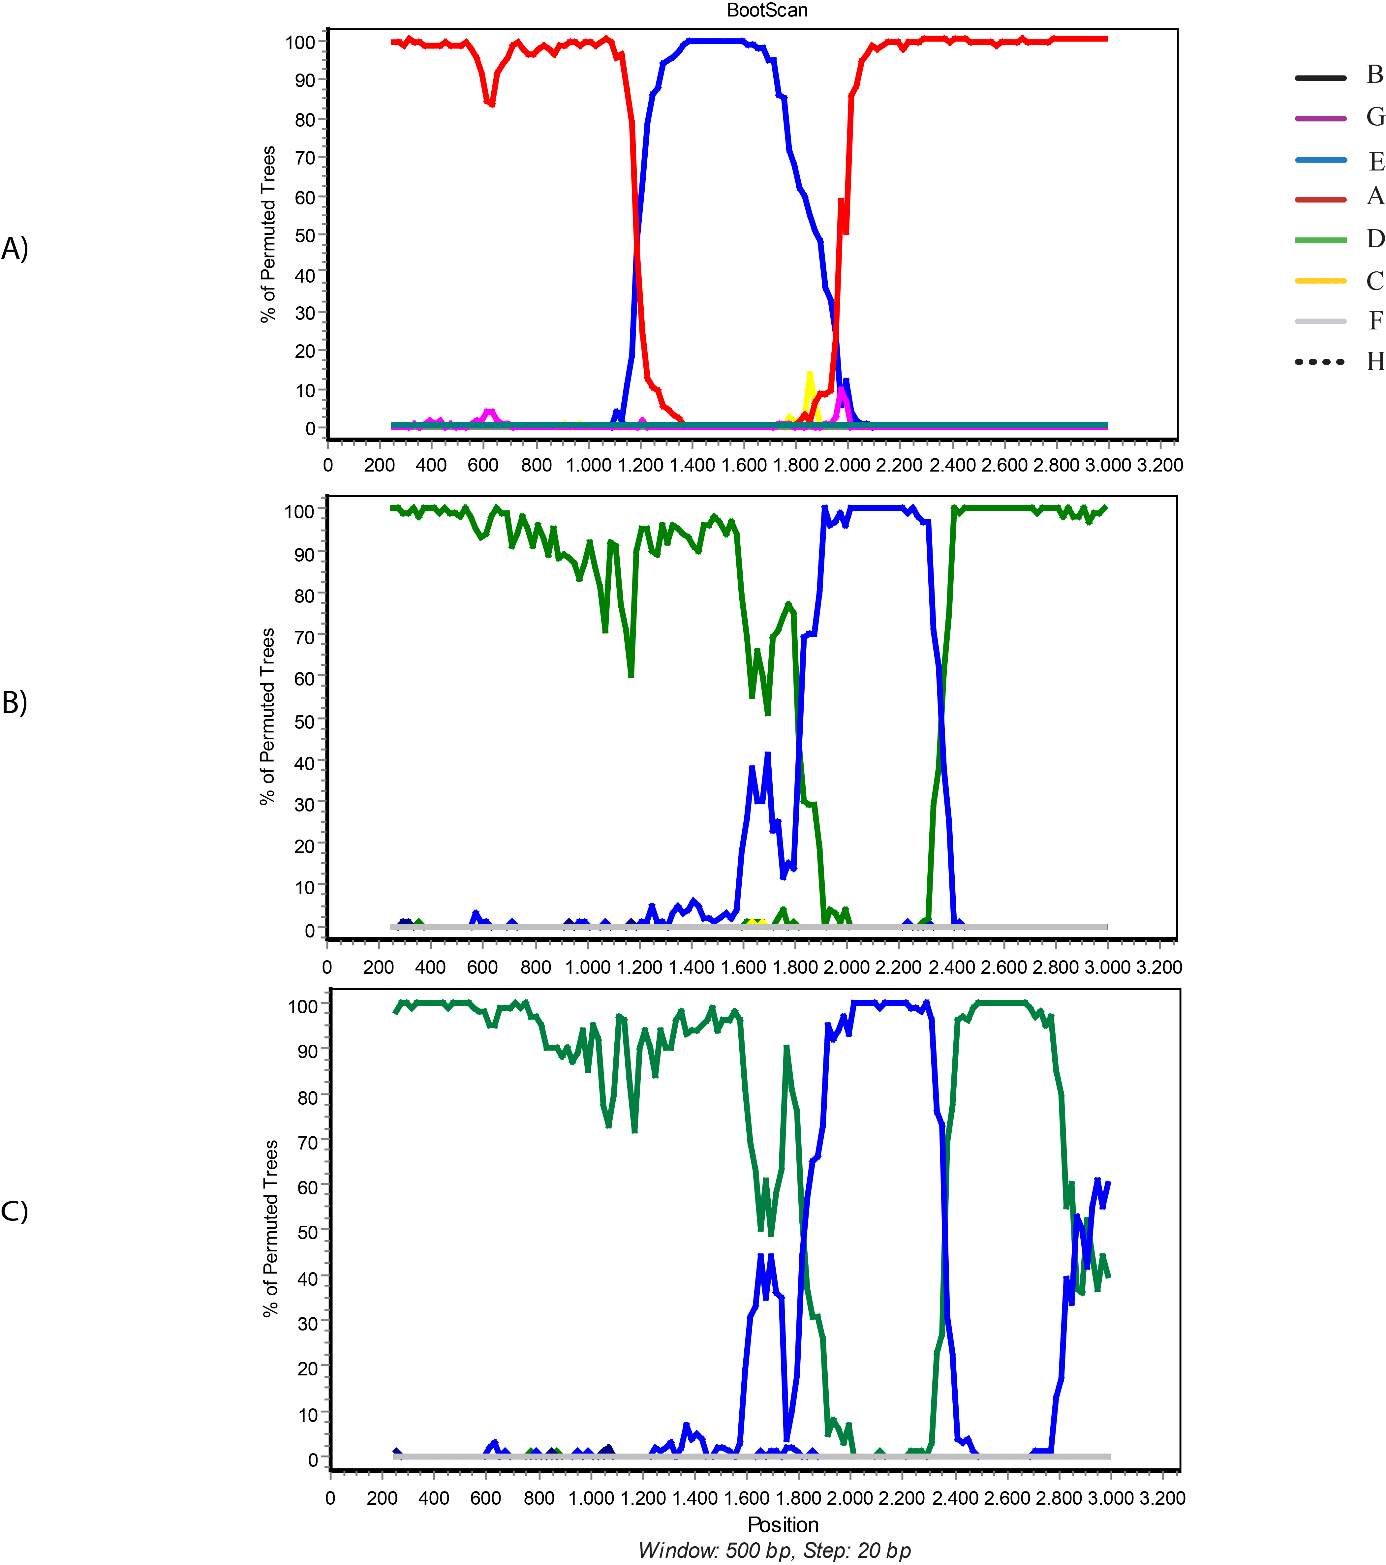
\includegraphics[width=.7\textwidth]{figs1}
    \caption[HBV BootScan results]{BootScan analysis of HBV isolates. We analyzed the complete genomes of the MB-58, MB-92, and MB-56 isolates of one patient from Guinea and two patients from Rwanda. The BootScan results reveal A) recombination between HBV genotypes A and E in one strain (MB-58), and in B) and C), recombination between HBV genotypes A and E in two other strains (MB-92 and MB-56, respectively).}
    \label{supfig:hbv-s1}
\end{figure}

\begin{figure}[!htbp]%
    \centering
    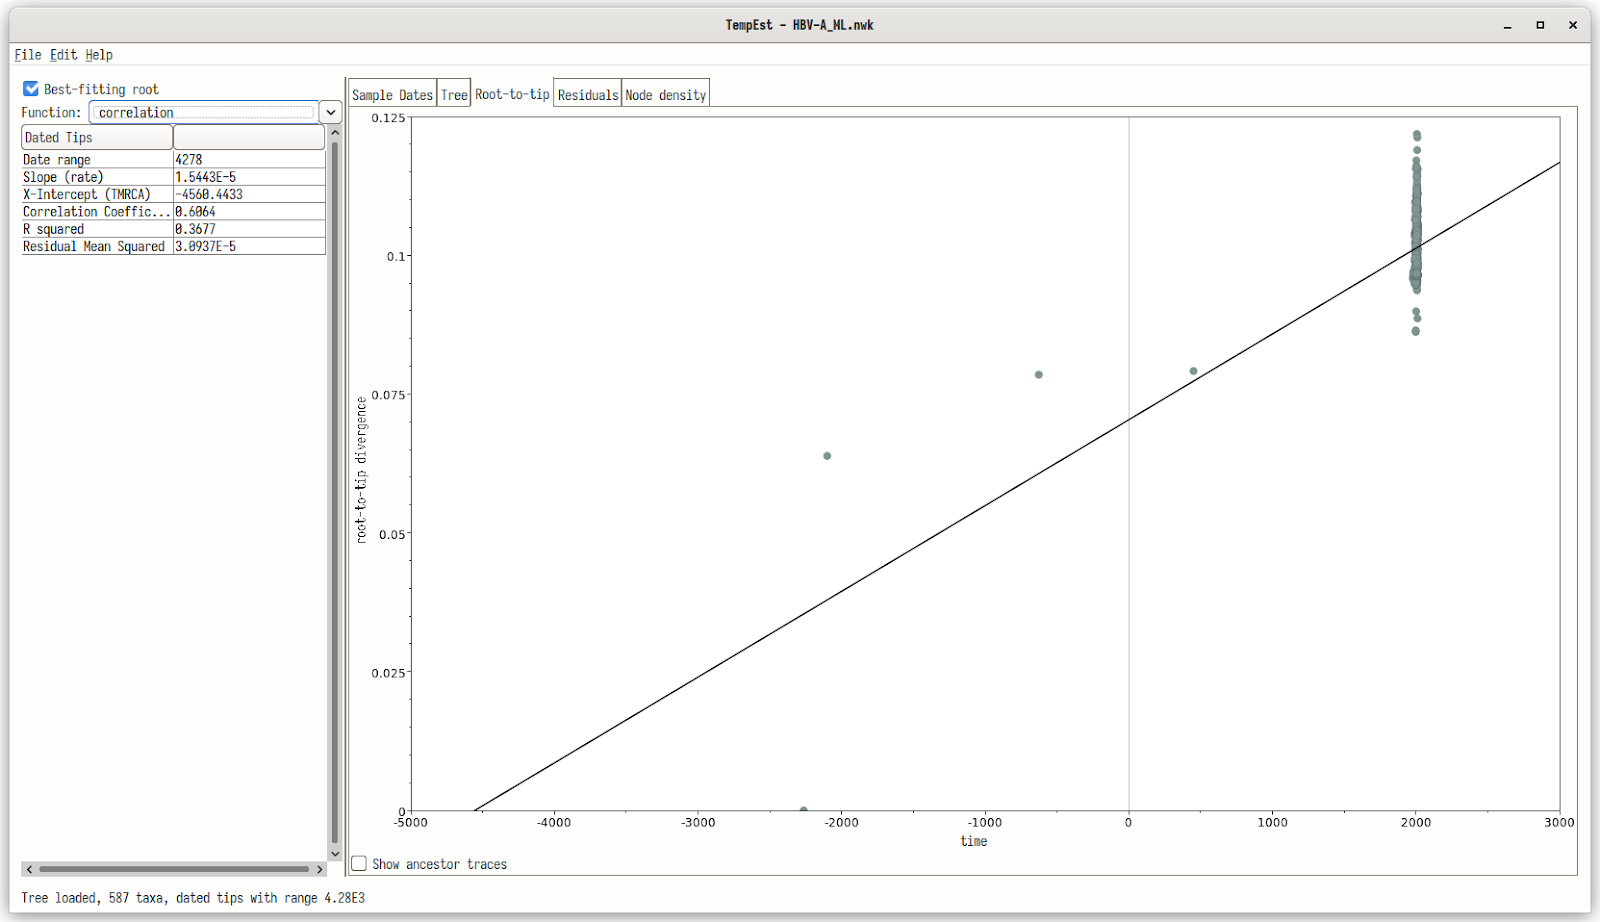
\includegraphics[width=\textwidth]{figs2}
    \caption[HBV-A temporal signal analysis]{Root-to-tip scatterplot of HBV-A sequences including ancient genomes, with estimated substitution rate overlaid. This represents the results of our initial maximum likelihood phylogenetic inference.}
    \label{supfig:hbv-s2}
\end{figure}

\begin{figure}[!htbp]%
    \centering
    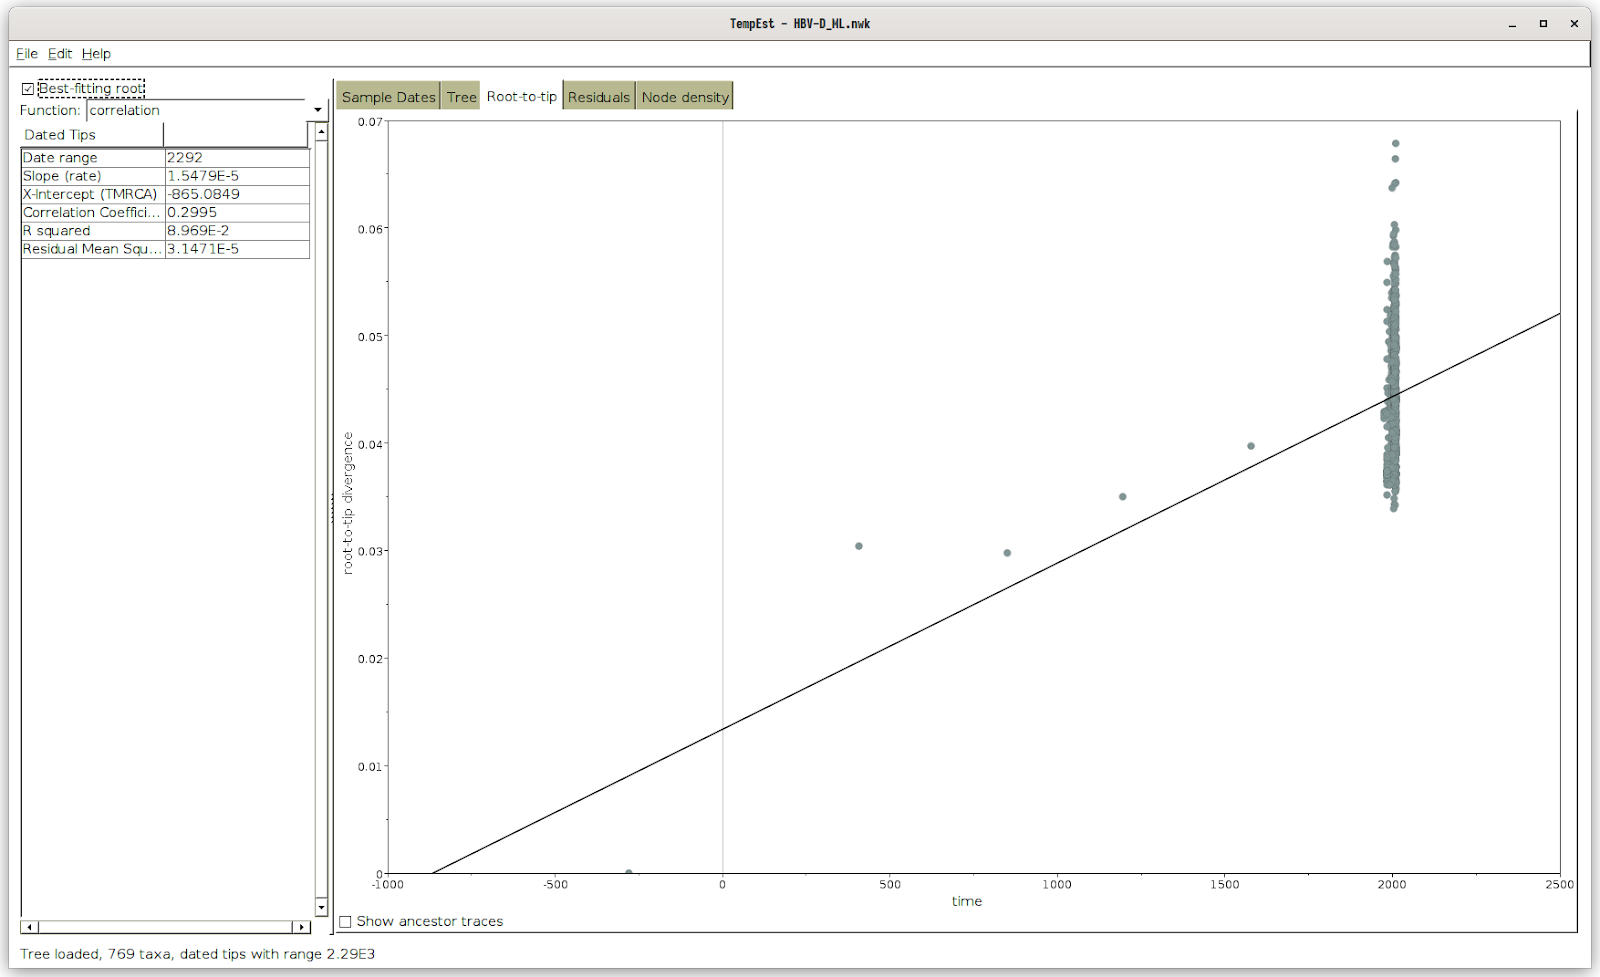
\includegraphics[width=\textwidth]{figs3}
    \caption[HBV-D temporal signal analysis]{Root-to-tip scatterplot of HBV-D sequences including ancient genomes, with estimated substitution rate overlaid. This represents the results of our initial maximum likelihood phylogenetic inference.}
    \label{supfig:hbv-s3}
\end{figure}

\begin{figure}[!htbp]%
    \centering
    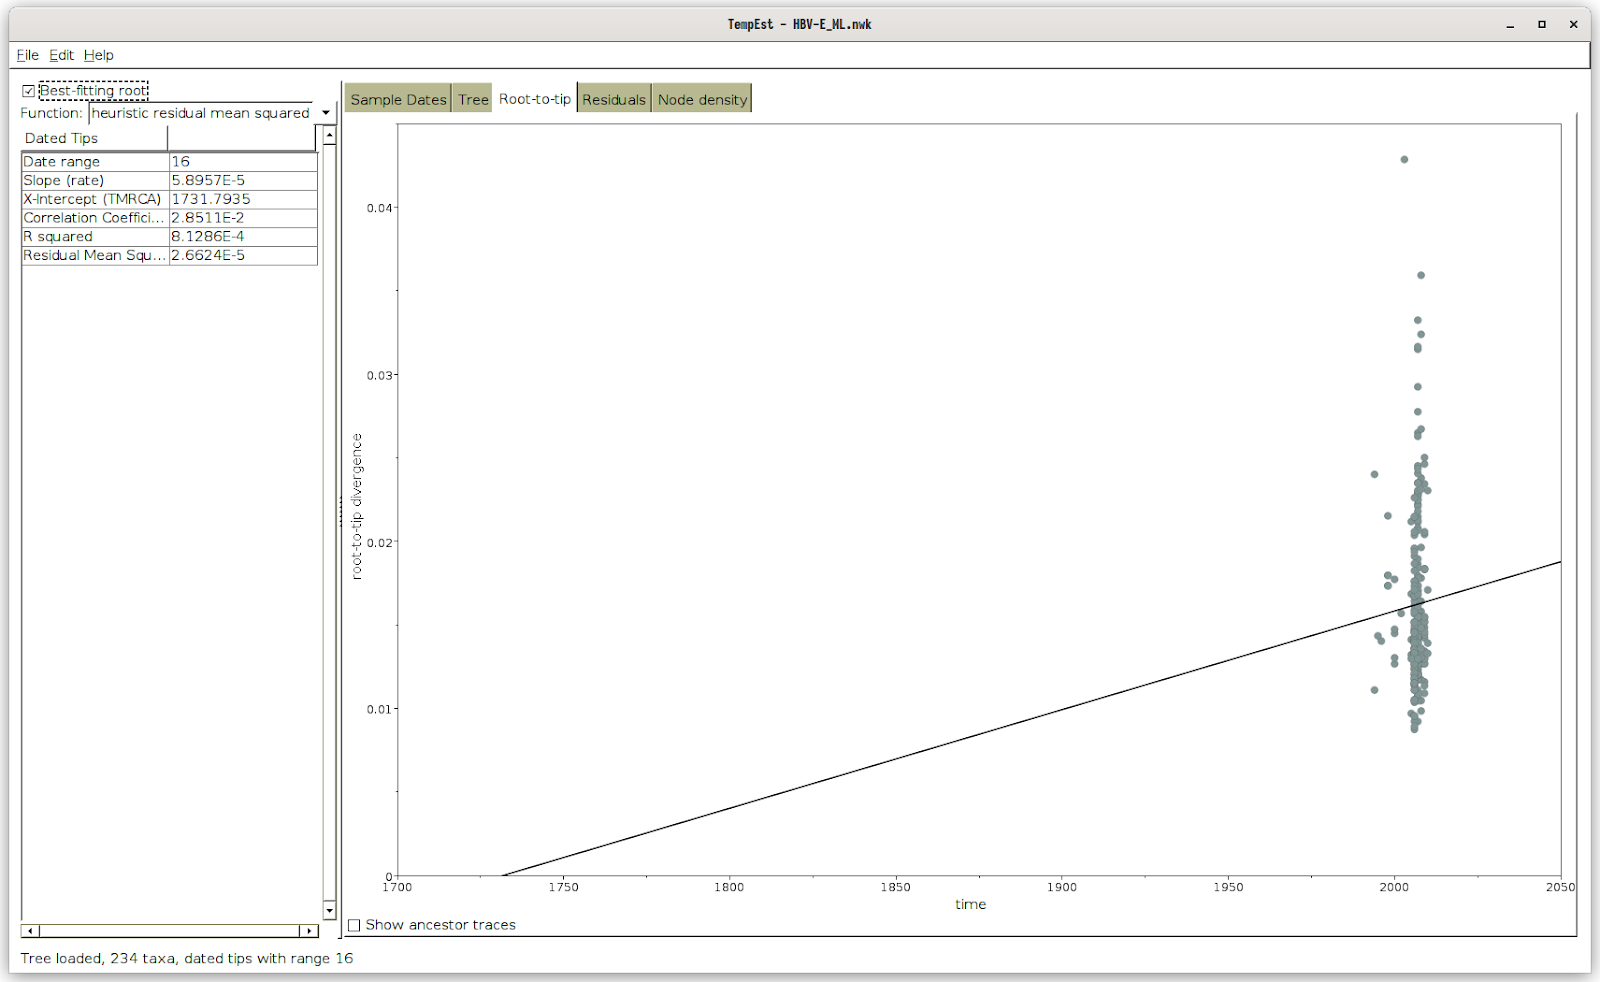
\includegraphics[width=\textwidth]{figs4}
    \caption[HBV-E temporal signal analysis]{Root-to-tip scatterplot of HBV-E sequences, with estimated substitution rate overlaid. This represents the results of our initial maximum likelihood phylogenetic inference.}
    \label{supfig:hbv-sX}
\end{figure}

%%%%%%%%%%%%%%%%%%%%%%%%%%%%%%%%%%%%%%%%%%%%%%%%%%
% Keep the following \cleardoublepage at the end of this file,
% otherwise \includeonly includes empty pages.
\cleardoublepage

% vim: tw=70 nocindent expandtab foldmethod=marker foldmarker={{{}{,}{}}}
